\documentclass[11pt, a4paper, oneside]{Thesis} % Paper size, default font size and one-sided paper
\usepackage[table,xcdraw]{xcolor}

\usepackage{wrapfig}
\usepackage{lscape}
\usepackage{rotating}
\usepackage{graphicx}
\usepackage{amsmath}
\usepackage{mdframed}
\usepackage{multirow}
\usepackage{algorithm}
\usepackage{algpseudocode}

% ADD DRAFT WATERMARK TO PAGES

% \usepackage{tikz}
% \usepackage[printwatermark]{xwatermark}
% \newsavebox\mybox
% \savebox\mybox{\tikz[color=red,opacity=0.3]\node{DRAFT};}
% \newwatermark*[allpages,angle=60,scale=7,xpos=-15,ypos=10]{\usebox\mybox}


%\usepackage{subcaption} %incompatible with subfig
\usepackage[square, numbers]{natbib} % Use the natbib reference package - read up on this to edit the reference style; if you want text (e.g. Smith et al., 2012) for the in-text references (instead of numbers), remove 'numbers' v

\hypersetup{urlcolor=black, colorlinks=true} % Colors hyperlinks in blue - change to black if annoyingv`	
\title{\ttitle} % Defines the thesis title - don't touch this





%======================================================================|
%\thesistitle{An Approach to Writing a Thesis\\[3mm] for MDes at IIITDM}
\thesistitle{An Unsupervised Video Summarization System}
\degree{B.Tech. Computer Engineering}
\authors{\textbf{Shivesh M. M.}}
\supervisor{Dr. Sivaselvan B}
\department{Department of CSE}
%======================================================================|

\tolerance=1
\emergencystretch=\maxdimen
\hyphenpenalty=10000
\hbadness=10000




%======================================================================|
\begin{document}
\makeatletter
\renewcommand*{\NAT@nmfmt}[1]{\textsc{#1}}
\makeatother

% prints author names as small caps


\frontmatter % Use roman page numbering style (i, ii, iii, iv...) for the pre-content pages

\setstretch{1.6} % Line spacing of 1.6 (double line spacing)

% Define the page headers using the FancyHdr package and set up for one-sided printing
\fancyhead{} % Clears all page headers and footers
\rhead{\thepage} % Sets the right side header to show the page number
\lhead{} % Clears the left side page header

\pagestyle{fancy} % Finally, use the "fancy" page style to implement the FancyHdr headers

\newcommand{\HRule}{\rule{\linewidth}{0.5mm}} % New command to make the lines in the title page

% PDF meta-data
\hypersetup{pdftitle={\ttitle}}
\hypersetup{pdfsubject=\subjectname}
\hypersetup{pdfauthor=\authornames}
\hypersetup{pdfkeywords=\keywordnames}

%----------------------------------------------------------------------------------------
%	TITLE PAGE
%----------------------------------------------------------------------------------------

\begin{titlepage}
\begin{center}


%\HRule \\[0.4cm] % Horizontal line
\vspace{0.4cm} % Horizontal line
{\huge \bfseries \ttitle}\\[0.4cm] % Thesis title
%\HRule \\[1.5cm] % Horizontal line
\vspace{1.5cm} % Horizontal line

 
 \large \textit{Project Report}\\[0.3cm] % University requirement text
\textit{Submitted by}\\[0.4cm]

\authornames\\[-2mm]\hspace{-0.2cm}\textbf{ (Roll No: COE16B034)}\\[-2.5mm]
\vspace{0.75cm}
in partial fulfilment for the award of the degree\\
	\vspace{0.75cm}
	\large {\bf Bachelor of Technology}\\
		\vspace{0.25cm}
	in\\
		\vspace{0.25cm}
	\large {\bf Computer Engineering}

\vfill
\graphicspath{ {./Figures/} }
\begin{figure}[hb]
  \centering
  
\includegraphics[width=0.35\linewidth]{iiitdm.png}
\end{figure}

\textsc{ \UNIVNAME}\\[1.5cm] % University name
\large \today\\[2cm] % Date


\end{center}

\end{titlepage}

%----------------------------------------------------------------------------------------
%	DECLARATION PAGE
%	Your institution may give you a different text to place here
%----------------------------------------------------------------------------------------

\Declaration{\addtocontents{toc}{\vspace{1em}} % Add a gap in the Contents, for aesthetics


% \begin{center}
% \LARGE{\underline{\textbf{Declaration of Originality}}}
% \end{center}
\noindent This is to certify that the project titled \textbf{"\ttitle"} submitted by \authornames
\noindent~to the \textbf{Department of 
Computer Engineering} at the \textbf{Indian Institute of Information Technology, 
Design and Manufacturing, Kancheepuram} for the award of
”Bachelor of Technology in Computer Engineering”, is a bonafide record of the project
work done under my supervision. The contents of the project, in full or in parts, have
not been submitted to any other Institute or University for the award of any degree.
%\noindent 

\vspace{20mm}
\noindent \textbf{Dr. B SIVASELVAN}\\[-2mm]
\vspace{1mm}

Project Guide
\vspace{1mm}

\noindent Assistant Professor\\
\noindent Indian Institute of Information Technology Design and Manufacturing Kancheepuram\\
\noindent Chennai 600127\\
\noindent India

\noindent Place : Chennai

\noindent Date : 13/03/2020

\vfill{}}

\clearpage % Start a new page






%----------------------------------------------------------------------------------------
%	ABSTRACT PAGE
%----------------------------------------------------------------------------------------

\addtotoc{Abstract} % Add the "Abstract" page entry to the Contents

\abstract{\addtocontents{toc}{\vspace{1em}} % Add a gap in the Contents, for aesthetics

Video summarization technique focuses on the task of generating concise and meaningful summaries of large video data/files. 

This project focuses on this emerging area in the context of educational videos of specific interest. The proposed summarization technique exploits the linguistic/spoken content in the video source data. This proposed model shall be of immense help to learners who want summarized and short but connected video content. 

The proposed model employs a customized tf-idf function. After applying this modified tf-idf function on individual subtitle entries treated as documents, and the subtitle file as a corpus, the entries are ranked based on the sum of the tf-idf values. 

The top ranked subtitle entries are chosen as per the requirement of the final summary length. Next, a novel parameter called the Flexibility Parameter, $F$ is introduced which smoothes out the short lengths of the selected clips by selecting unchosen clips if the number of unselected clips between any two unchosen clips is at most F. 

Finally, the consecutive contiguous clips are identified, the final clips are cropped out and stitched using \texttt{ffmpeg} library.
}

\clearpage % Start a new page

%----------------------------------------------------------------------------------------
%	ACKNOWLEDGEMENTS
%----------------------------------------------------------------------------------------

\setstretch{1.3} % Reset the line-spacing to 1.3 for body text (if it has changed)

\acknowledgements{\addtocontents{toc}{\vspace{1em}} % Add a gap in the Contents, for aesthetics

I would like to convey my sincerest thanks to people who have made this project possible. First and foremost I would like to convey my heartfelt gratitude to my parents without whom none of this would have been possible.

Further, I would like to extend my genuine thanks to my project guide and supervisor, Dr. B Sivaselvan whose guidance and advice were instrumental in making this project a reality. I am fortunate to have got an opportunity to obtain his expertise and knowledge which were monumental to this project

Finally, I am thankful to the TA's of Dr. Sivaselvan who have helped me with timely help and advice.
}
\clearpage % Start a new page

%----------------------------------------------------------------------------------------
%	LIST OF CONTENTS/FIGURES/TABLES PAGES
%----------------------------------------------------------------------------------------

\pagestyle{fancy} % The page style headers have been "empty" all this time, now use the "fancy" headers as defined before to bring them back

\lhead{\emph{Contents}} % Set the left side page header to "Contents"
\tableofcontents % Write out the Table of Contents

\lhead{\emph{List of Figures}} % Set the left side page header to "List of Figures"
\listoffigures % Write out the List of Figures

\lhead{\emph{List of Tables}} % Set the left side page header to "List of Tables"
\listoftables % Write out the List of Tables

%----------------------------------------------------------------------------------------
%	ABBREVIATIONS
%----------------------------------------------------------------------------------------

% \clearpage % Start a new page

% \setstretch{1.5} % Set the line spacing to 1.5, this makes the following tables easier to read

% \lhead{\emph{Abbreviations}} % Set the left side page header to "Abbreviations"
% \listofsymbols{ll} % Include a list of Abbreviations (a table of two columns)
% {
% \textbf{FEA} & \textbf{F}inite \textbf{E}lement \textbf{A}nalysis \\
% \textbf{FEM} & \textbf{F}inite \textbf{E}lement \textbf{M}ethod \\
% \textbf{LVDT} & \textbf{L}inear \textbf{V}ariable \textbf{D}ifferential \textbf{T}ransformer \\
% \textbf{RC} & \textbf{R}einforced \textbf{C}oncrete
% %\textbf{Acronym} & \textbf{W}hat (it) \textbf{S}tands \textbf{F}or \\
% }

%----------------------------------------------------------------------------------------
%	PHYSICAL CONSTANTS/OTHER DEFINITIONS
%----------------------------------------------------------------------------------------
%
%\clearpage % Start a new page
%
%\lhead{\emph{Physical Constants}} % Set the left side page header to "Physical Constants"
%
%\listofconstants{lrcl} % Include a list of Physical Constants (a four column table)
%{
%Speed of Light & $c$ & $=$ & $2.997\ 924\ 58\times10^{8}\ \mbox{ms}^{-\mbox{s}}$ (exact)\\
%% Constant Name & Symbol & = & Constant Value (with units) \\
%}

%----------------------------------------------------------------------------------------
%	SYMBOLS
%----------------------------------------------------------------------------------------

% \clearpage % Start a new page

% % \lhead{\emph{Symbols}} % Set the left side page header to "Symbols"

% % \listofnomenclature{lll} % Include a list of Symbols (a two column table)
% % {
% % $D^{el}$ & elasticity tensor \\
% % $\sigma$ & stress tensor \\
% % $ \varepsilon $ & strain tensor \\
% % % Symbol & Name & Unit \\

% % }

%----------------------------------------------------------------------------------------
%	DEDICATION
%----------------------------------------------------------------------------------------
%
\setstretch{1.3} % Return the line spacing back to 1.3
%
\pagestyle{empty} % Page style needs to be empty for this page
%
% \dedicatory{For/Dedicated to/To my\ldots} % Dedication text
%
\addtocontents{toc}{\vspace{2em}} % Add a gap in the Contents, for aesthetics

%----------------------------------------------------------------------------------------
%THESIS CONTENT - CHAPTERS
%----------------------------------------------------------------------------------------
\mainmatter % Begin numeric (1,2,3...) page numbering
\pagestyle{fancy} 



\chapter{Introduction} 
\label{Chapter1} 
\lhead{Chapter 1. \emph{Introduction}} 

    With the rapid proliferation of electronic gadgets, there's a remarkable growth in the amount of textual and non-textual data generated by every individual. Further, the sudden surge in the availability of multiple video-on-demand platforms like Hotstar, Amazon Prime Video, Netflix, and YouTube has led to an exponential increase in the amount of visual content generated. 
    
    About 500 hours of video is uploaded every minute to YouTube, and this rate of growth is only accelerating. In addition to this, users watch upwards of 1 billion hours of content every day \cite{Youtube_2019}. So far, the research on multimedia data has been majorly on extracting the statistics and syntactic details of data. There are plenty of methods available to extract the objective content from the data like recognizing objects or scenes, finding the motion of the objects, but there is not much contribution on extracting the semantic context of a video. In recent times, the research interest has shifted towards unveiling the semantic context of the data. Many deep learning approaches concentrate on extracting the semantic context of the data such as emotion recognition, summarization, etc. 
	
	Though video-sharing and streaming platforms like YouTube and Netflix\cite{netflix} have advanced recommendation systems powered by the behavior of users and their dwell time on videos, the downside is that users are becoming selective of what they see and prefer to know the substance of the content beforehand \cite{youtube}. Thus, paired with the fact that users are spending increasingly less time watching videos it becomes important to convey the content as quickly as possible with as little filler content as possible. This has sparked a rise in approaches to "summarize" content, aiming to reduce the length of the video besides retaining the informativeness and perception quality of the video. Video summarization is categorized into static and dynamic approaches. Static approaches are keyframe based that results in a storyboard summary. But the temporal evolution of the video is lost in the process of extracting the keyframes which highlight the important scenes of the video. On the contrary, dynamic approaches preserve the temporal evolution besides skimming the highlights from the video. 
	
	Summarizing a long sequenced video has many applications in scenarios where time is a critical resource. As summarized video is expected to contain the essence of the whole video, it is highly beneficial for academicians on educational platforms to revisit a topic. Further, summarizing a video ensures that the cognitive load on the minds of learners is minimized. Work done by Brame \textit{et. al.} in \cite{brame2015effective} describes multiple types of mental effort necessary to assimilate video-form educational content. This paper discusses the additional unwanted cognitive impact called \textit{Extraneous load} which makes video understanding harder due to malformed lessons, or poorly structured content. 
	
	In another paper by Guo \textit{et. al.} which analyzed over \textbf{6.9 million video sessions} over four MOOC courses on eDX to map student engagement with length of the videos. Their findings also point to the fact that shorter videos are more engaging with normalized engagement time close to 100\% till the 6 minutes to 9 minute range and progressively falling off thereafter \cite{guo2014video}.

	
	Thus video summarization serves a very important purpose for educational video comprehension. It will also be useful for general public to be informed about the summarized News headlines for a week or a month. Now, the complexity lies in knowing what constitutes importance in a video. The importance and topic relevance are subjective and differs from person to person. Moreover, another challenging fact is the highly diversified unstructured content which makes the semantic understanding difficult.

\chapter{Literature Survey} 
\label{Chapter1_2} 
\lhead{Chapter 2. \emph{Literature Survey}} 

\section{Video summarization using deep semantic features 
\texorpdfstring{\cite{otani_2016_video}}{}}
%			\begin{mdframed}
%				\textbf{Paper Title: }\textit{Video summarization using deep semantic features}
%			\end{mdframed}

%			
			\begin{figure}[ht]
				\centering
					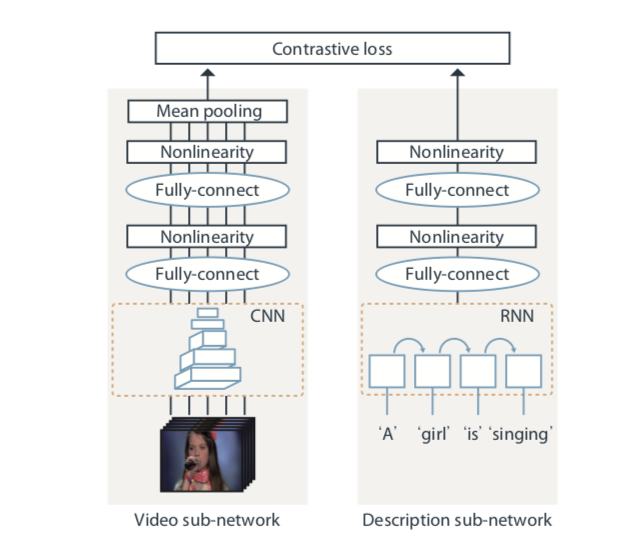
\includegraphics[width=0.5\textwidth]{P1Arch}
				\caption{Deep Semantic Architecture}
				\label{fig:p1arch}
			\end{figure}
			
			
			\subsection{Major Ideas}
				 This paper discusses creating of video summaries using uniformly extracted video segments.
				 
				 Current video suggestion systems according to the paper, \cite{otani_2016_video}, suggest videos based on video metadata, like title, user tags, descriptions, and thumbnails. This is primarily up to the user to specify them.

				As a result if the metadata is misleading, it can lead to completely wrong predictions, as the content of the video is disregarded in current prediction systems.
				
				Further they point to many alternatives that make use of low level visual features that cannot handle various concepts except a predefined set of concepts. Further, videos in real life tend to be of a varied nature, 
				
			\subsection{Input, Processing and Outputs}
				
				\textit{\underline{Input}}
					\begin{itemize}
						\item This uses a temporal sliding window, where the window is shifted by 1 second. 
						\item Each segment, \(V\) was re-sampled at 1 frame per second, so \(V\) has five frames. Thus the video segments run at 1 frame per second. 
						\item In comparison, most modern videos have anywhere between 24 (cinematic) to 60 frames per second (handheld video). Even higher framerates are possible with top of the smartphones and high end video recorders.
					\end{itemize}
				\textit{\underline{Processing}}
					
					The processing pipelined implemented is a DNN, a Deep Neural Network, which utilizes two sub-networks to map a video and its description to a common semantic space and jointly train them using a large-scale dataset.
					
					This video sub-network is a CNN, while the description network is an RNN network. Both these networks are mapped down to a common semantic space and trained using contrastive loss (this method of loss is a distance based loss instead of a error based loss function)
					\begin{align}
						loss(X_n, Y_n) &= t_nd(X_n, Y_n) + (1 - t_n) max(0, \alpha - d(X_n, Y_n))\\
						t_nd &= 1,\ if\ (X_n,Y_n) > 0 \\
						t_nd &= 0,\ otherwise
					\end{align}
					\(d(X_n, Y_n)\) is the squared Euclidean distance between Xn and Yn.
					
					The video sub-network is a modified version of VGG10, modified in order to fit this problem better. A fully connected classification layer has been replaced with two fully connected layers with \texttt{tanh} activation and finally using a mean pooling layer.
					
					Further, the text network uses a Skip-Thought Vector design proposed by Kiros \textit{et al.} \cite{Kiros_2015}
					
				\textit{\underline{Output}}
				
					Visualizing the 2D plot of deep features from a video shows that similar segments are closer in the semantic space and thus applying the solution to the k-medoids problem. This implemented using a parameter, K, that represents the length of the video summary required
					
					Given the set of deep features extracted, k-medoids thus finds and returns the subset of video segments, S, that minimizes:
					
					\begin{align}
						F(S) = \sum_{X\in X}min_{s\in S}||X-S||^2
					\end{align}
				Where the optimal subset is 
					\begin{align}
						S^* = argmin_SF(S)
					\end{align}
					
\section{Content Summarization with content-based Recommender System \texorpdfstring{\cite{jiang_2019_comprehensive}}{}}
%			\begin{mdframed}
%				\textbf{Paper Title: }\textit{Comprehensive video understanding: Video summarization with content-based video recommender design}
%			\end{mdframed}
	\begin{figure}[ht]
	\centering
		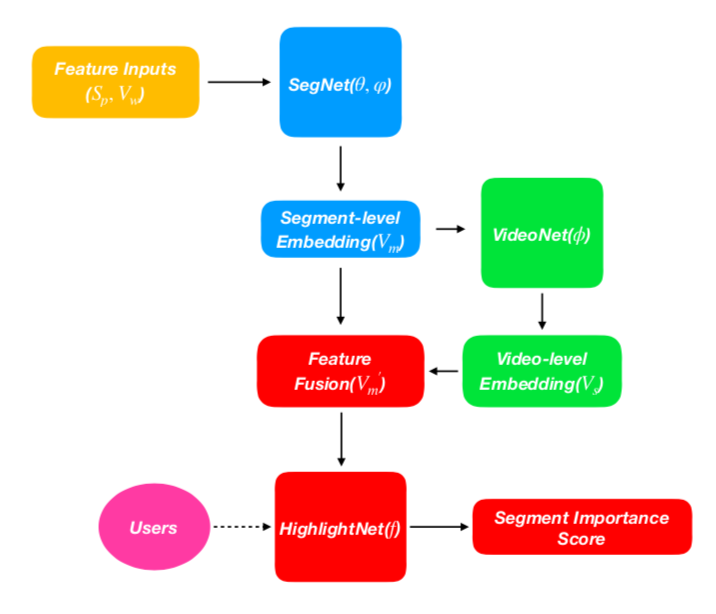
\includegraphics[width=0.5\textwidth]{P2Arch}
	\caption{Recommender Based Architecture}
	\label{fig:p2arch}
    \end{figure}
	
    \subsection{Major Ideas}
    	This paper posits that one of the main challenges in video summarization is with regards to subjectivity, different people may have different selections on what makes an important segment for a video.
    	
    	Key Ideas tackled in this paper are (verbatim from the paper):
    	
    	\begin{enumerate}
    		\item Unifying various inputs on different semantic levels to one framework by formatting video summarization into a recommender problem.
    		\item Developing an algorithm that models independent segments and segment sequence (whole video).
    		\item Extend the summarisation framework with self-supervised learning and data augmentation to deal with the lack of labelled data. (This is a valuable contribution as it enables the system to learn with data that would be more common in real life.)
    	\end{enumerate}
	
    \subsection{Input, Processing and Outputs}
    	
    	\textit{\underline{Input}}
    	
    		This problem models the video summarization task as a video recommendation system wherein each segment is treated as an entity to "recommend". 
    		
    		The input is a set of video segments and the target importance score of each segment.
    		
    	\textit{\underline{Processing}}
    	
    		This uses three subnetworks to learn multiple functions in order to facilitate prediction. 
    		
    		\begin{align}
    			L(f) = L(f(\varphi(\theta(S_p),V_w) \oplus\phi(\varphi(\theta(S_p),V_w))))
    		\end{align}
    		
    		The three subnetworks,
    		
    		\begin{enumerate}
    			\item SegNet will learn \(\theta\) and \(\varphi\)
    			\item VideoNet will learn \(\phi\)
    			\item HighlightNet will learn f
    		\end{enumerate}
    		
    		The video segments are also shuffled often to ensure that the correct segments are determined without focussing on when it occurs in the video.
    		
    	\textit{\underline{Output}}
    
    		By training various models (ResNet50, ResNet152, GoogleNet) on various datasets (ImageNet, and CoView2019), they propose a table comparing the performance.
    		
    		All of the models perform comparably, with their summary score in the range of 80.83 to 81.81. 
			
\section{TruNet: Story Preserving Truncation \texorpdfstring{\cite{yang_2019_trunet}}{}}
    \begin{figure}[ht]
    	\centering
    		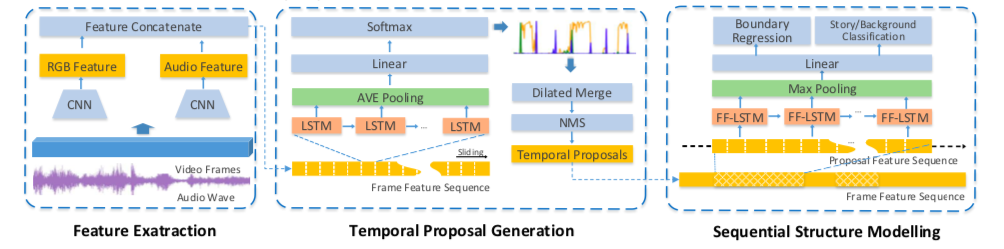
\includegraphics[width=\textwidth]{P3Arch}
    	\caption{TruNet Architecture}
    	\label{fig:p3arch}
    \end{figure}
    			
    \subsection{Major Ideas}
    	This paper points out that although much progress has been made in video highlight detection and video summarization, many of the them focus on producing a coherent whole story in the final combined highlight and there is no requirement of an unbroken story to each sub-video.
    	
    	They develop a large dataset called TruNet, with 1470 videos and a total of 2101 hours of content. The average video length is longer than one hour.
    	
    	These videos are from a variety of sources, like talk shows, TV shows, and reality shows.
    	
    	Their contribution is threefold:
    	
    	\begin{enumerate}
    		\item Introduction of a new practical problem in video truncation
    		\item Collection and annotation of a new large dataset for studying this problem, which can become a complementary source to existing video datasets
    		\item Proposal of a baseline framework that involves a new temporal proposal generation module and a new sequence modeling module, with better performance compared to traditional methods.
    	\end{enumerate}
    
    \subsection{Input, Processing and Outputs}
    	
    	\textit{\underline{Input}}
    	
    		\begin{itemize}
    			\item The paper proposes a custom dataset called the TruNet. On the other hand, the ActivityNet, even though it has more videos, the length of videos is very small, averaging at 2 minutes.
    			\item TruNet proposed by the paper has an average video length of 80 minutes.
    			\item This data is sourced from a wide varying range of content, including talkshows, tv shows, and reality shows.
    		\end{itemize}
    		
    	\textit{\underline{Processing}}
    	
    		The processing methodology is two fold. 
    		
    		\begin{enumerate}
    			\item \textbf{Boundary Aware network:} This is a novel network that takes in 7 consecutive frames as an input to an LSTM and uses the output as an input to a MaxPooling layer and finally a linear layer. \\ It outputs the probabilities of whether these are within the “story” (or the summary),  or background. \\ It also outputs the Story beginning boundary probability and Story ending boundary probability.
    			\item \textbf{FF-LSTM:} For learning, they stack multiple traditional LSTM layers with skip connections running between them. This is called the Fast Forward LSTM (FF-LSTM) \\ These added connections have no non-linear activations nor recurrent computations. Thus, information is propagated easily. \\ Finally a MaxPooling layer is used to average the outputs.
    		\end{enumerate}
    		
    		After computing the intersection over unions (IoU). If \(<\)0.3 then the sample is negative, and if \(>\)0.7 the sample is a positive sample.
    		
    		The BAN network is trained using SGD with momentum 0.9, epoch number 70, decay at 0.0005 and a mini batch size of 256 on four K40 GPUs.
    		
    	\textit{\underline{Output}}
    		For evaluation purposes, the paper computes a mean average precision (mAP) value at three different IoU thresholds, \{0.5,0.7,0.9\}
    		
    		A comparison has been done with state of the art video summary methods, \textbf{vsLSTM} and \textbf{HD-VS}.
    		
    		For different values of the IoU thresholds, \(\alpha\), they showcase that that their model performs consistently better than their alternatives w.r.t. to the mAP values.\cite[Page 8]{yang_2019_trunet}
    		
% \section{Video Summarization and Scene Detection
% by Graph Modeling \texorpdfstring{\cite{graph}}{}}
%     \begin{figure}[ht]
%     	\centering
%     		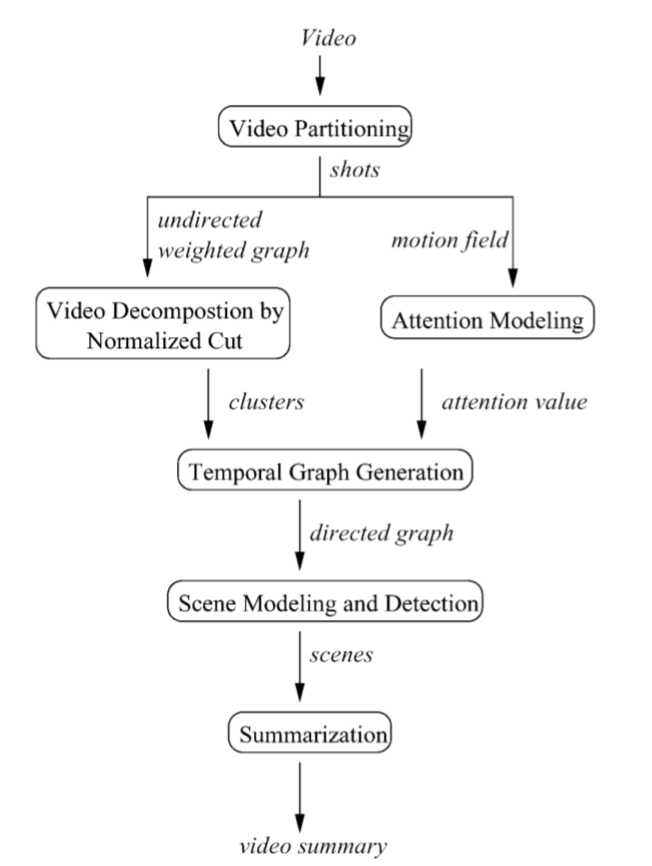
\includegraphics[width=0.4\textwidth]{Ngo}
%     	\caption{Architecture}
%     	\label{fig:ngo}
%     \end{figure}
    			
%     \subsection{Major Ideas}
%         The work in \cite{graph} summarizes video based on entropy, perceptivity and skim ratio. 
        
%         The video is depicted as a temporal graph and this graph is sliced into video clusters by using the normalized cut algorithm.
        
%         These video clusters that are temporally partitioned contains a series of shots with similar visual content. Further, an adaptive keyframe selection and construction scheme is used to select an optimal keyframe from each cluster. 
        
%         This approach takes into account the motion of the objects and the visual setting as a key factor for summarization and excludes captions and spoken text which is expected to reveal semantic details. 
        
%         Results state that with a 75\% cut-off from the original content, 20\% of the information is lost. 
		
%     \subsection{Input, Processing and Outputs}
    	
%     	\textit{\underline{Input}}
    	
%     		\begin{itemize}
%     			\item
%     		\end{itemize}
    		
%     	\textit{\underline{Processing}}
    		
%     		\begin{enumerate}
%     			\item
%     		\end{enumerate}
    		
%     	\textit{\underline{Output}}
    		
% Chapter Template

\chapter{Proposed Video Summarization System - Modeling \& Implementation} % Main chapter title

\label{Chapter3} % Change X to a consecutive number; for referencing this chapter elsewhere, use \ref{ChapterX}

\lhead{Chapter 3. \emph{Proposed Video Summarization System - Modeling \& Implementation}} % Change X to a consecutive number; this is for the header on each page - perhaps a shortened title
\makeatletter
\def\BState{\State\hskip-\ALG@thistlm}
\makeatother
%----------------------------------------------------------------------------------------
%	SECTION 1
%----------------------------------------------------------------------------------------

\section{Project Pipeline}

\begin{figure}[ht]
	\centering
		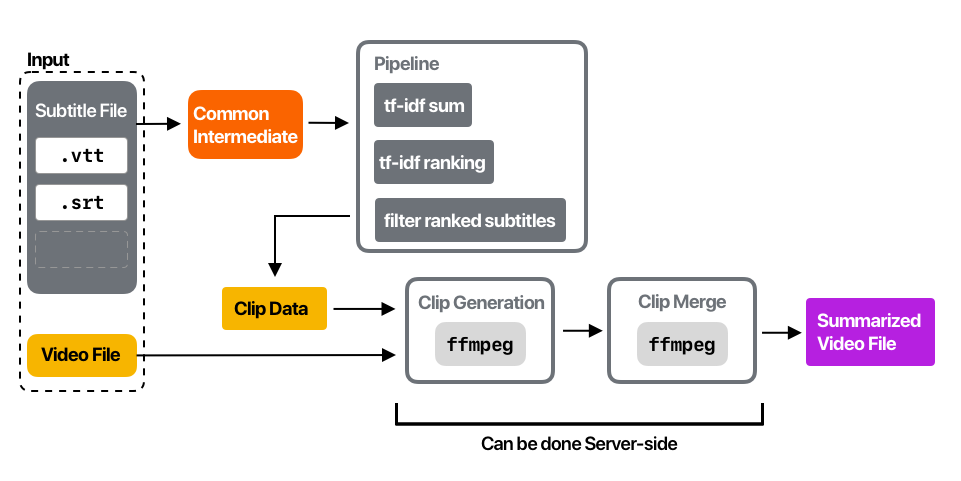
\includegraphics[width=\textwidth, keepaspectratio=true]{Graphic}	
		\caption{Current Pipeline}
		\label{currentpipeline}
\end{figure}

\section{Implementation}

This project creates a video summary taking into account multiple video features. The fact that subtitles are ever-present in videos of today especially in long form videos that warrant summarization, significantly eases this task. Academic videos specifically from portals like NPTEL, Coursera and other MOOC platforms make use of lecture transcriptions in order to facilitate learning which can be easily leveraged in order to enable summarization. 
			
	\subsection{Subtitle Parsing}	
		The current implementation leverages these embedded subtitles by supporting both kinds of popular \verb|.srt| and \verb|.vtt| files extracted from the video. Further, auto-generated YouTube captions can also be utilized for the second module.
			
		The first module takes in the subtitle files, (\verb|.srt| and \verb|.vtt|) and parses them into an intermediate file. This ensures that the text learning module can be run independent of the subtitle format. The intermediate incorporates the subtitle entry length, one-indexed subtitle entry (\verb|.srt| includes indices while \verb|.vtt| lacks indices). The subtitle file reading is chunked to efficiently handle large subtitle files and preventing the whole file from loading onto the memory.
		
		Normally, with long form videos, due to the length of the video, subtitles are often auto-generated by the video hosting provider, e.g. NPTEL videos often utilize auto-generated video subtitles using YouTube due to manual captions being prohibitively hard to implement. These auto-generated video subtitles are generated using a voice to text engine that runs server-side. The subtitle parser can also parse these autogenerated video captions and work on summarization using that, thereby requiring no manual subtitle file input and working off the automatically generated subtitle file.
			
	\subsection{Text Learning}
		Now the second module is invoked which works on the intermediate file generated by the subtitle parser. Common intermediate file is loaded, then punctuation is stripped. Further common English stop words are removed and the subtitle entry string is lemmatized using a \verb|WordNet Lemmatizer|. Next a tf-idf vectorizer is called upon this data which returns the tf-idf matrix.
			
		Summing the tf-idf matrix across columns gives us a column matrix with one cell for each subtitle entry representing the tf-idf sum of the words in the subtitle.
		
		\begin{algorithm}
		\caption{Choosing video clips based on tf-idf sums}
		\label{naivealgo}
		\textbf{Input:} Target length, $t$ and the list of Clip data, $L$ 
		\textbf{Output:} $chosen\_L$, such that $chosen\_L \subseteq L$ and total duration $\leq t$
		\begin{algorithmic}[1]
			\Procedure{GetClips}{}
				\State $t \leftarrow \text{Target clip length}$
				\State $L \leftarrow \text{List of clips}$
				\State $idx \leftarrow 0$
				\State $chosen\_L \leftarrow []$
				\State $L \leftarrow decreasing(L, L['tf\_idf'])$	 \Comment{Sort in decreasing order based on tf-idf values}
				\BState start:
				\If {$t < 0$} 
					\State \Return \textit{chosen\_L}
					\State \textbf{stop}
				\EndIf
				\State $t \leftarrow t - L[\textit{idx}].duration$
				\State $chosen\_L.append(L[idx])$
				\State $idx \leftarrow idx + 1$
				\State \textbf{goto} \textit{start}
			\EndProcedure
		\end{algorithmic}
	\end{algorithm}
			
		Since, the parser module also returns the duration of a subtitle, arranging it in descending order and summing up the durations till it exceeds the required length gives the subtitle entries to include in the final output video (as shown in Algorithm~\ref{naivealgo}).
	    
	    \begin{algorithm}
		\textbf{Input:} Naively chosen clips, $chosen\_L$ and the Flexibility Parameter, $F$ 
		
		\textbf{Output:} A flexibly extended list of clips, $Flex\_L$, such that $chosen\_L \subseteq Flex\_L \subseteq L$.
		\caption{Extend naively chosen clips with clips selected using Flexibility Parameter}
		\label{FParamAlg}
		\begin{algorithmic}[1]
			\Procedure{ExtendSelection}{}
				\State $selected \leftarrow []$		
				\State $idx \leftarrow 0$
				\State $len\_selected \leftarrow len(chosen\_L)$
				\BState indexLoop:
					\If{$L[idx]$ in $chosen\_L$} \State $selected.append(idx)$
					\EndIf
					\State $idx \leftarrow idx + 1$
					\If{$idx < len(chosen\_L)$} \State \textbf{goto} \textit{indexLoop}
					\Else \State \textbf{goto} \textit{main}
					\EndIf
				\BState main:
					\State $idx \leftarrow 0$
					\State $Flex\_L \leftarrow selected$
					\State \textbf{goto} \textit{loop}
					\BState loop:
						\If {$selected[ idx + 1] - selected[idx]\leq F~\&\&~selected[idx+1] - selected[idx] > 1$}
							\State $Flex\_L.append([selected[idx]+1 \hdots selected[idx + 1])$
						\EndIf
						\If{$idx \leq len(selected) - 2$}
							\State $idx \leftarrow idx + 1$
						\Else
							\State \textbf{stop}
						\EndIf
			\EndProcedure
		\end{algorithmic}
	\end{algorithm}
	    
    	\subsubsection{Flexibility Parameter}
    		Now the concept of a flexibility parameter is introduced. This is depicted in the Figure~\ref{flexparam}, where the green entries indicate the initially selected subtitle entries based on the tf-idf sum ranking. 

            The process of selecting this Flexibility Parameter is described in Algorithm~\ref{FParamAlg}.
            
    		Based on the value of the flexibility parameter, say \(N\), selected subtitle entries with \(\leq N\) unselected entries in between are also selected.
    				
    		Setting the parameter to zero generates a summary that's as close as possible to the required length. Whereas, setting the parameter to a large value will include the whole video.
    				
    				\begin{figure}[ht]
    				\centering
    					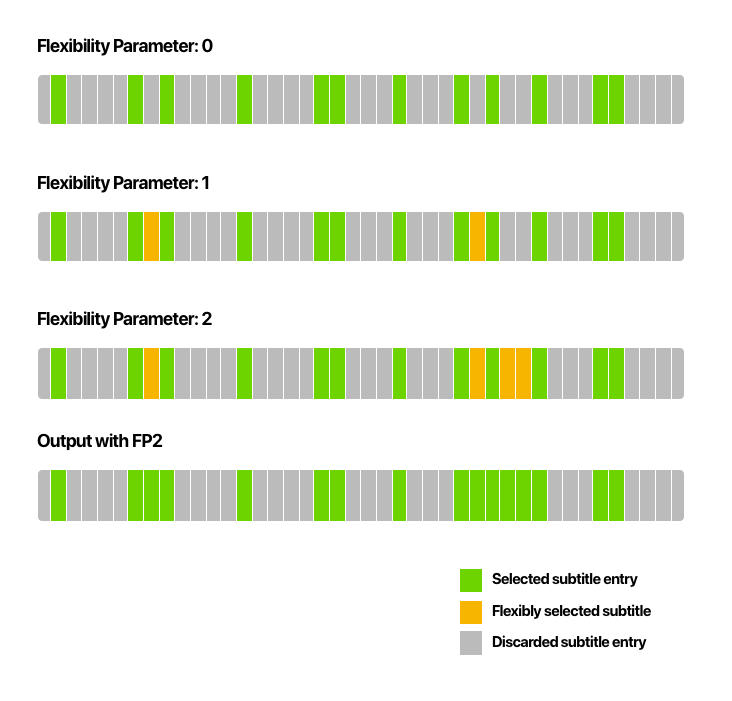
\includegraphics[width=0.5\textwidth, keepaspectratio=true]{Flexibility}	
    					\caption{Flexibility Parameter}
    					\label{flexparam}
    				\end{figure}
    				
    				\begin{mdframed}
    					\textbf{\underline{Need}}
    					
    						The concept of flexibility parameter tackles the fundamental idea that if two subtitle entries close by are important then the subtitles between them are important enough to be included in the summary.
    						
    						This also ensures that the final output is smoother and is not jarring to view. As a result of the flexibility parameter, the final video output becomes longer than the required length.
    				\end{mdframed}
    			This module creates another intermediate file with the start time, end time and the index of the clips to cut and join to create the summary. 
		
		\subsection{Clip and Summary Creation}	
			Now the final module takes in the intermediate clip data and parses it. It takes in the time stamps and rounds it. The subtitle entries in the original subtitle file have exact times (down to microseconds) to start showing subtitles and to stop showing the subtitles. This is removed when the start times are floored down and the stop times are ceiled up. 
			
			\begin{algorithm}
		\caption{Algorithm to get contiguous sequences of clips}
		\label{contiguous}
		\textbf{Input:} Indices of the subtitle file chosen, $chosen$
		\textbf{Output:} A list of lists $sets\_of\_clips$, consisting of contiguous sequences of clip data.
		
		\begin{algorithmic}[1]
			\Procedure{ContiguousClips}{}
				\State $idx \leftarrow 0$
				\State $sets\_of\_clips \leftarrow []$
				\State $temp \leftarrow []$
				\BState loop:
					\If{$chosen[idx]~\textbf{not in}~temp$}
						\State $temp.append(chosen[idx])$
					\EndIf
					
					\If {$chosen[idx+1]-chosen[idx] == 1$}
            			\State $temp.append(chosen[idx+1])$
            			\State \textbf{continue}
			        \Else
			            \State $sets\_of\_clips.append(temp)$
			            \State $temp \leftarrow []$
					\EndIf
					\If{$idx \leq len(selected) - 2$}
							\State $idx \leftarrow idx + 1$
						\Else
						    \State \textbf{return} \textit{sets\_of\_clips}
							\State \textbf{stop}
						\EndIf
			\EndProcedure
		\end{algorithmic}
	\end{algorithm}
			
			Further, contiguous sequences of clips are identified and taken together in order the determine the start and the end time of the final clip using Algorithm~\ref{contiguous}. Thus, if say the subtitle entries with indices $1,2,3,4$ are selected, then this ensures that the start time of 1 and the end time of 4 are taken for the purposes of cropping the video.
			
			Next the multiprocessing module calls \verb|ffmpeg| running parallel on the processor of the computer. Finally the created subclips are merged together, again using \verb|ffmpeg| to create the output. \verb|ffmpeg| uses hardware acceleration to encode video streams (For example, h264\_videotoolbox and h265\_videotoolbox are Apple's GPU access API on macOS and \verb|nvenc| for nVidia GPUs).
			
			\begin{mdframed}
				\textbf{\underline{Advantages}}\\
					Since the clip creation and summary generation is running independent as long as the video and the subclip intermediate is available, the initial generation can be done on-device and then the heavy work can be run completely server side leveraging large parallel processing power.
			\end{mdframed}
	
	\subsection{Audio Processing}
	    The audio processing pipeline consists primarily of the following steps:
	    
	    \begin{enumerate}
	        \item \textbf{Audio Extraction:}
	            This step involves extracting the audio waveform file from the input video, into it's constitutent audio file and video file.
	        \item \textbf{Audio Pre-processing:}
	            This step is implemented using the \texttt{ffmpeg} library and selectively encoding the audio track to a separate \texttt{.wav} file in order to enable processing.
            \item \textbf{Audio Feature Extraction:}
                This process involves extracting features from the exported audio file. Explored feature extraction techniques include:
                \begin{itemize}
                    \item \textbf{MFCC:} Mel Frequency Cepstral Coefficient are Coefficients of the Mel-frequency spectrum that resemble how a human hears audio, with high emphasis on lower frequencies and lower emphasis on high frequencies.
                \end{itemize}
            \item \textbf{Learning from Audio:} This process involves mining information from the extracted audio file. Multiple kinds of information can be extracted from the audio track.
                \begin{itemize}
                    \item Emotion Detection and Energy Detection
                    \item Voice activity detection
                \end{itemize}
            Work is being done to determine which will serve most suitable to the purposes of enhancing video sumamrization with additional cues.
	    \end{enumerate}
% Chapter Template

\chapter{Results and Discussions} % Main chapter title

\label{Chapter4} % Change X to a consecutive number; for referencing this chapter elsewhere, use \ref{ChapterX}

\lhead{Chapter 4. \emph{Results and Discussions}} % Change X to a consecutive number; this is for the header on each page - perhaps a shortened title

%----------------------------------------------------------------------------------------
%	SECTION 1
%----------------------------------------------------------------------------------------

	The Table~\ref{stellar} and Table~\ref{nptel} show the results for evaluating this project on different platforms and configurations. Utilizing the \texttt{ffmpeg} command line video library for this task allows the use of hardware acceleration to encode video streams (For example, \texttt{h264\_videotoolbox} and \texttt{h265\_videotoolbox} are Apple's GPU access API on macOS, \verb|nvenc| for Nvidia GPUs and \texttt{OpenCL} is used for cross platform access). 
	
	Further the Graphs~\ref{fig:stellar} and \ref{fig:nptel} plot the sum of the tf-idf values of the selected subtitles and the subtitle index. This shows a clear demarcation between selected and unselected subtitle indices.
	
	Further, as this implementation is run on multiple threads determined by the processor of the host machine, this saves a considerable amount of time, so much so that the parallel implementation of this program run on a CPU competes on par with the serial implementation on a GPU as shown in the \texttt{nvenc} row in Table~\ref{stellar}.
	
	 This method of summarization also has the added advantage of extensive modularity. By performing the initial textual tf-idf parsing on device, the actual video clipping and summary generation can be implemented server-side, delivering the final edited videos to the users. As the video cropping and stitching is done on server side and is not required in the first place for pre-processing, storage space is also saved. Thus, the proposed approach saves time and space and works with vastly improved efficiency. Unlike deep learning methods, this approach is devoid of parameters and hence no time is invested in building and training a model. 

		\begin{table}[!htp]
		\caption{Results for a sample 9 minute educational video chosen from youtube}
		\label{stellar}
\resizebox{\columnwidth}{!}{\begin{tabular}{|c|c|c|c|c|c|c|}
\hline
S. No              & Video Title                                            & Video Length              & Flex. Param.       & Video Segments      & Quality                & Bitrate                \\ \hline \hline
\multirow{7}{*}{1} & \multirow{7}{3cm}{How to Move the Sun - Stellar Engines} & \multirow{7}{*}{9 m 00 s} & \multirow{5}{*}{2} & \multirow{5}{*}{15} & \multirow{2}{*}{1080p} & \multirow{2}{*}{5094k} \\
                   &                                                        &                           &                    &                     &                        &                        \\ \cline{6-7} 
                   &                                                        &                           &                    &                     & \multirow{3}{*}{480p}  & \multirow{3}{*}{750k}  \\
                   &                                                        &                           &                    &                     &                        &                        \\
                   &                                                        &                           &                    &                     &                        &                        \\ \cline{4-7} 
                   &                                                        &                           & \multirow{2}{*}{3} & \multirow{2}{*}{11} & \multirow{2}{*}{480p}  & \multirow{2}{*}{750k}  \\
                   &                                                        &                           &                    &                     &                        &                        \\ \hline
\end{tabular}}\vspace{5mm}
\resizebox{\columnwidth}{!}{\begin{tabular}{|l|l|l|l|l|l|}
\hline
Encoder            & Bitrate & Text Learning Time (s) & Video gen. Time (s)                   & Time (mins)                   & Final Length of Output                                       \\ \hline \hline
h264\_videotoolbox & default &\multirow{7}{*}{2.12} & 687                        & 11 m 27s                       &                                                    \\ \cline{1-2}\cline{4-5}
default            & default &  & 1041                       & 17 m 21s                       &                                                    \\ \cline{1-2}\cline{4-5}
default            & 750k    & & 130                        & 2 m 10s                        &                                                    \\ \cline{1-2}\cline{4-5}
h264\_videotoolbox & default & & 83                         & 1 m 23s                        &                                                    \\ \cline{1-2}\cline{4-5}
h264\_videotoolbox & 750k    & & 109                        & 1 m 49s                        &                                                    \\ \cline{1-2}\cline{4-5}
nvenc (serial)     & 750k     & & 109                        & 1m 49s                         & \multirow{-6}{*}{3 m 11 s}                         \\ \cline{1-2}\cline{4-6}
nvenc (serial)     & 750k     & & \cellcolor[HTML]{67FD9A}78 & \cellcolor[HTML]{67FD9A}1m 18s & \cellcolor[HTML]{67FD9A}                           \\ \cline{1-2}\cline{4-5}
h264\_videotoolbox & 750k     & & \cellcolor[HTML]{67FD9A}61 & \cellcolor[HTML]{67FD9A}1 m 1s & \multirow{-2}{*}{\cellcolor[HTML]{67FD9A}3 m 54 s} \\ \hline
\end{tabular}}
\end{table}

\begin{figure*}[!htpb]
\centering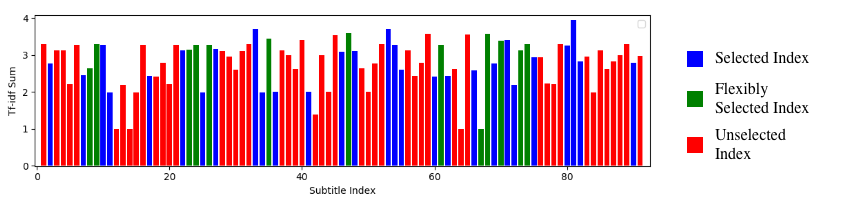
\includegraphics[width=\textwidth]{Legend}
\caption{Plot of selected, flexibly selected indices and unselected indices and their Tf-idf sums for the video from Table~\ref{stellar}}
\label{fig:stellar}
\end{figure*}

\begin{table}[!htpb]
\caption{Results for a 26 minute educational video chosen from NPTEL}
\label{nptel}
\resizebox{\columnwidth}{!}{\begin{tabular}{|c|c|c|c|c|c|c|}
\hline
S. No & Video Title           & Video Length & Flex. Param. & Video Segments & Quality & Bitrate \\ \hline
1     & Hypothesis testing-II & 26 m 24 s    & 10           & 29             & 1080p   & 896k    \\ \hline
\end{tabular}}\vspace{5mm}
\resizebox{\columnwidth}{!}{\begin{tabular}{|l|l|l|l|l|l|}
\hline
Encoder            & Bitrate & Text Learning Time (s) & Video gen. Time (s)          & Time (mins)                       & Final Length of Output           \\ \hline
h264\_videotoolbox & 750k    & 2.63                   & \cellcolor[HTML]{67FD9A}1451 & \cellcolor[HTML]{67FD9A}24 m 11 s & \cellcolor[HTML]{67FD9A}9 m 29 s \\ \hline
\end{tabular}}
\end{table}

\begin{figure*}[!htpb]
\centering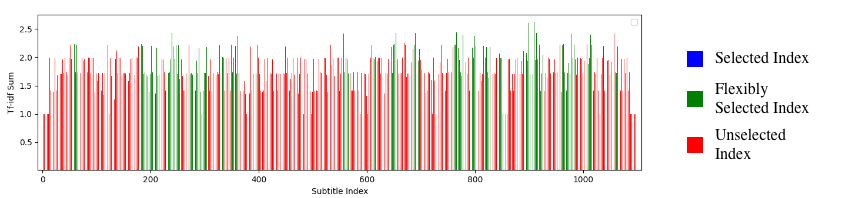
\includegraphics[width=\textwidth]{NPTEL}
\caption{Plot of selected, flexibly selected indices and unselected indices and their Tf-idf sums for the video from Table~\ref{nptel}}
\label{fig:nptel}
\end{figure*}
% Chapter Template

\chapter{Conclusions and Extensions} % Main chapter title

\label{Chapter5} % Change X to a consecutive number; for referencing this chapter elsewhere, use \ref{ChapterX}

\lhead{Chapter 5. \emph{Conclusions and Extensions}} % Change X to a consecutive number; this is for the header on each page - perhaps a shortened title

%----------------------------------------------------------------------------------------
%	SECTION 1
%----------------------------------------------------------------------------------------

This project thus has implemented an efficient approach to video summarization, coming up with succinct and quality summaries of large videos especially with an appropriate choice of the flexibility parameter, $F$ using a modified Tf-idf method and a parallel approach to video processing and clip generation.

		\begin{figure}[!ht]
			\centering
				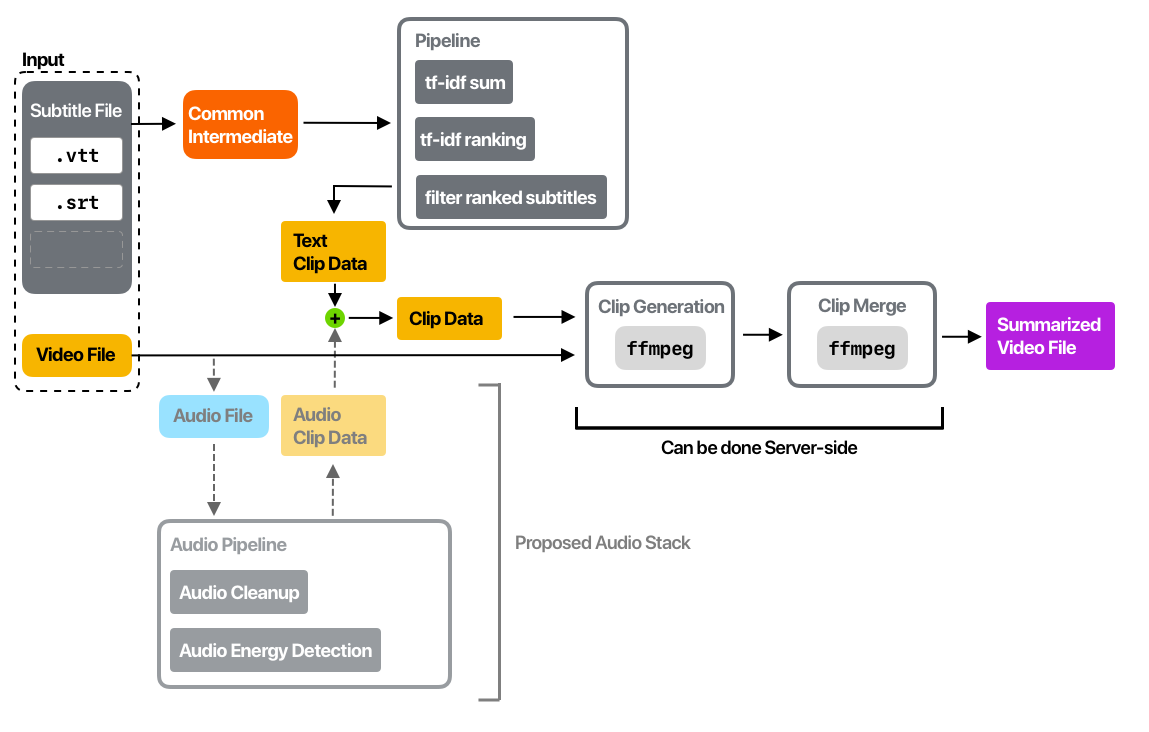
\includegraphics[width=0.8\textwidth, keepaspectratio=true]{Future}	
				\caption{Future Pipeline}
				\label{futurepipeline}
		\end{figure}

\begin{itemize}
			\item Completion of the implementation of the audio processing pipeline.
			\item Generation of subtitles for the final video.
			\item Determining the optimum value of the Flexibility Parameter, $F$ for the optimum summary length.
			\item Jarring cuts in video is to be minimized. This can be done by appropriately choosing the parameter \(N\) and implementing crossfade filters and other transitions in \verb|ffmpeg|.
		\end{itemize}

%\input{chap_6} 
%\input{chap_7} 

%----------------------------------------------------------------------------------------
%THESIS CONTENT - APPENDICES
%----------------------------------------------------------------------------------------
% \addtocontents{toc}{\vspace{2em}} 
% \appendix 
% \input{app_1}
% \input{app_2}
% \input{app_3}

\addtocontents{toc}{\vspace{2em}} % Add a gap in the Contents, for aesthetics

\backmatter

%----------------------------------------------------------------------------------------
%BIBLIOGRAPHY
%----------------------------------------------------------------------------------------
\nocite{*}
\label{Bibliography}

\lhead{\emph{Bibliography}} % Change the page header to say "Bibliography"

\bibliographystyle{IEEEtran} % Use the "custom" BibTeX style for formatting the Bibliography

\bibliography{bibliography} % The references (bibliography) information are stored in the file named "Bibliography.bib"

\end{document}  
